%---Linda

The post processing is based on the correction of the measurement data.
The first part of the processing the measured data are processed with the corresponding data of the base station data to get a higher accurancy of the GPS data.
The nearest base station is Statens Kartverks SatRef located on Platåberget with a distance between 14 km and 20 km depending on the mass balance stake.
In the following text the mass balance stake is only named as stake and the pole with the Trimble receiver will be shortend to the name rover.
The second part of the processing contains the stake correction based on the measurements.
\medskip

In the previous reports the post processing was done with the commercial software Trimble Business Center (TBC). 
In this report we use a new method for the post processing. 
This method is an open source (OS) alternative which is available for different system softwares and ist useable without a license. 
The TBC is only available on a windows system and needs a licens.
This leads to a limitation in the application. 
We operate both methods to quantify if the TBC method can be replaced by the OS method.

\subsection{Trimble}

While the TBC post processing all mentioned steps from section 5 in Gölles (2012) are done.
For each day the data file from the measurements and the corresponding base station data file is imported. 
The data are available for the days of year(doy) 070, 072, 074 and 075.
All data files from the base station are in the .o18-format and downloaded from the server of Statkat server.
The data from the rover have the .t02 format. 
After the TBC post processing the results from the are stored in a .csv-file.
\medskip

The GNSS processing in the TBC use the combination of base station and rover data.
The goal is to “fix” the number of whole wavelengths between the rover and satellites.
This process is done in two steps by generating a 'float' solution an and resolve an integer value, the interger ambiguty. 
If a solution is sucessfully find it is defined as 'fixed'.
The transition from 'float' to 'fixed' is the initialization period.
A slow convergence of the solution is possible for longer baselines or when the signal is shield by objects in the surrounding.
After some amount of time the float solution can switch instantaneously to a fixed solution.
There is also a disadvantage of the float and fixed approach for integer ambiguity resolution.
At some point in time the convergence to fixed solution is hold on and impossible to change.
By mistake it is possible that during the post processing process a wrong fixed values is hold. 
Due to imposiibility to change the final value an unnormal high position error is possible. 
The result define then a wrong position, which is caused by a incorrect set of interger ambiguties.
During the processing the TBC use automatically the best way to measure and correct the position data. 
Mostly it is subdiveded in short and long baselines.
Baselines are determined by the distance between rover and base station.
For longer baselines the uncertainties have to be reduced with an additional approach, like a model.
For different settings and situations the TBC used different approaches for the tropospheric and ionospheric uncertainties and choose automaticly the right combinaion \citep{Trprocess}.
Therefore it is difficult to distinguish the settings used for the TBC post processing to compare with the open source processing.

\subsection{Open source}
The OS post processing requires different processing steps.
First of all the raw data file has to be transformed from the original Trimble format .t02 to the .tdg-format, because .t02-files are not readable for the final OS post processing program.
This transformation was done with the programm runpkr00 which is available on the website of unavco \url{http://kb.unavco.org/kb/article/trimble-runpkr00-v5-40-latest-version-mac-osx-10-7-windows-xp-7-linux-solaris-744.html}.
The used command is 
\begin{verbatim} 
runpkr00 -g -d filename.t02 
\end{verbatim}.
Due to problems with the package it was necessary to do a manual transformation of the package.
To provide the correct file format for the last post processing step we use the toolkit teqc.
This toolkit is also available on the website of unavco \url{https://www.unavco.org/software/data-processing/teqc/teqc.html}.
Then the file can be converted to an observation (.obs) and navigation (.nav) file by the commad
\begin{verbatim}
./teqc +nav filename.nav +obs filename.obs filename.tgd.
\end{verbatim} 
After this step it is necessary to download the base station data from the server of Statkart \url{http://ftp.statkart.no/}.
\medskip

The final step in the OS post processing of the GPS data is done with the open source program package RTKLIB.
This package is available for the download in the website \url{http://www.rtklib.com/rtklib.htm}.
In this package we use the executable rtkpost.exe in the subdirectory \textit{/bin} of the downloaded full package with source Programs with the version 2.4.2.
In this software the two navigation file from the receiver and the base station as well as the observation file from the receiver has to be read in.
For this method the .n18-format from the base station is needed as comparable navigation file. 
To exexute RTKPOST it is required to adjust the appropriate settings.
For all stakes the settings in the post processing were the same.
The settings are displayed in the header of the output file.
The header with the settings for the OS post processing is available in the appendix.
The setting are as similar as possible to the TBC settings.
But due to the automatical adjusment to the best correction in the TBC it is difficult to find the same set of settings.
In the OS post processing it is possible to select different correction methods for the tropospheric and ionospheric correction. 
Due to missing informations from TBC the probaly best method was choosen with 'broadcast' correction for the ionosphere and the 'saastamoinen' correction for optimize the accurancy due to tropospheric errors. 
The other settings can be taken from the header information to repeat the OS post processing. 
The final output after the post processing is a position file (.pos). 
The results of the OS post processing are given as a time series of latitude, longitude and elevation, where the horizontal components are transformed to the UTM coordinate system. 
Because the UTM coordinate system is consitenly uses in our report the coordinate transformation to UTM is done with a python function.
To get one position, including northing, easting an elevation value in m, the weighted mean over all time steps is calulated.
\medskip

Without the correction of the base station data the vaules for northing, easting and elevation fluctuate with a high frequency due to a lot of distrbances (compare subsection \ref{GPS:subsec:methods}). 
Exemplary this time series is shown in figure \ref{GPS:fig:T1-i_nocorr} for the first measurement of the stake T1-2017.
For the better understanding of the OS values it is usefull to compare timeseries of the post processed position values for two measurements at the same stake on differnet days.
In the first measurement (see figure \ref{GPS:fig:T1-i_timeseries}) the values converge after a few seconds to a fixed solution.
In the second measurement (see figure \ref{GPS:fig:T1-ii_timeseries}) the values vary during the hole time series without any tendency.
The properties of the second measurement leads to a bigger difference between the TBC value and the OS value.
A comparison to the whole time series of the TBC post processing is not possible, because it is not possible to get this out of the TBC.

\begin{figure}[H]
    \centering
    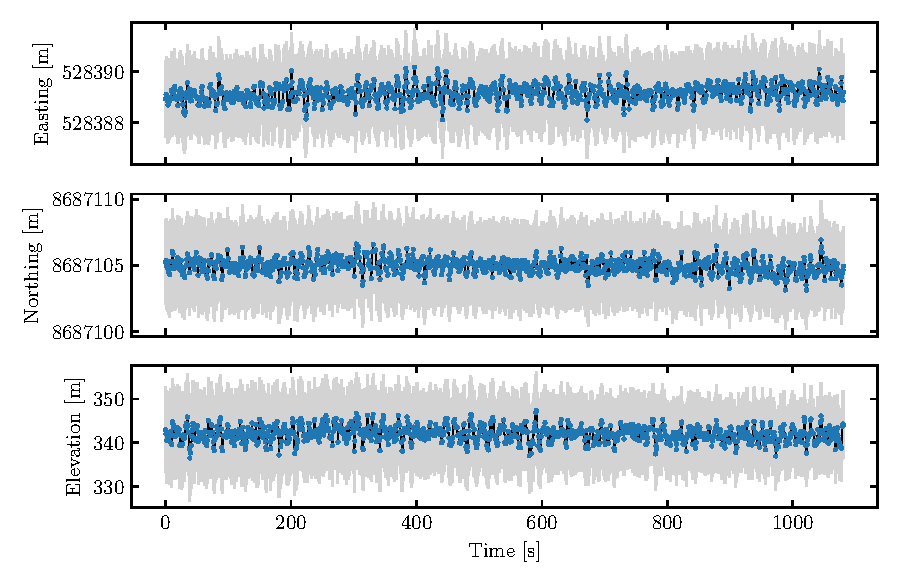
\includegraphics[width=\textwidth]{./figs/timeseries/46250700_org-T1-i-2017_Timeseries-east-north-elev.pdf}
    \caption{First of two measurements of position of stake T1-2017 without the correction by the base station data. The blue points are the open source values Northing, Easting and Elevation in m in respect to the measurement time in s. The solid black line connect the data points. The gray shadowed range shows the uncertainty area.}
    \label{GPS:fig:T1-i_nocorr}
\end{figure}

\begin{figure}[H]
    \centering
    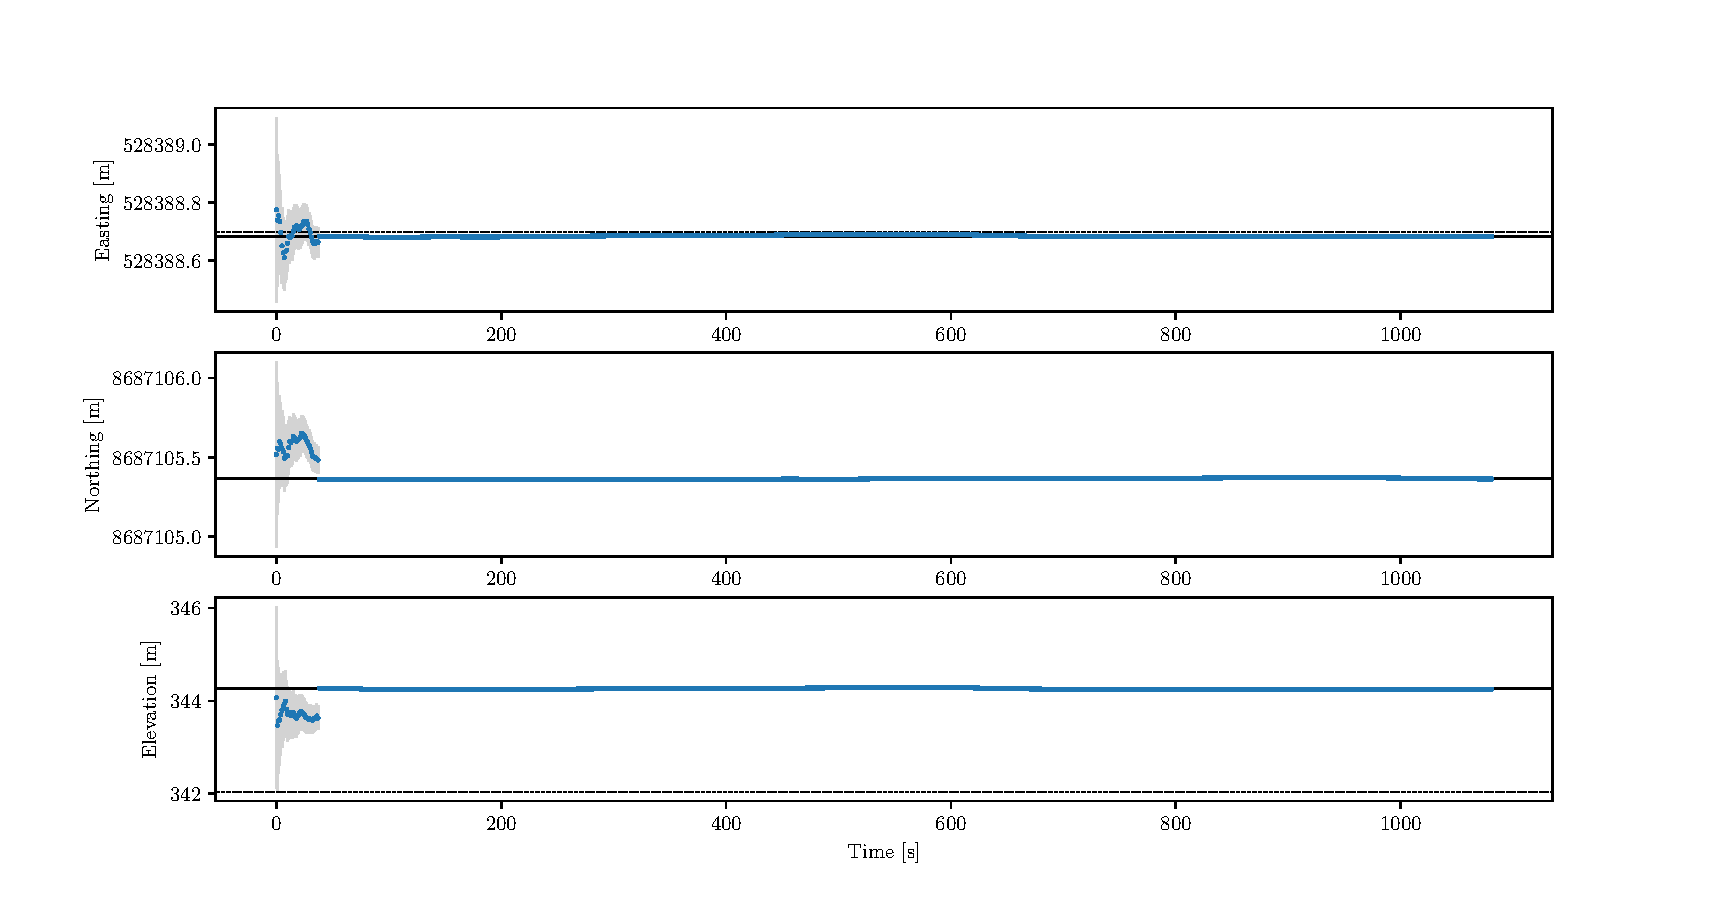
\includegraphics[width=\textwidth]{./figs/timeseries/46250700_corr-T1-i-2017_Timeseries-east-north-elev.pdf}
    \caption{First of two measurements of position of stake T1-2017 after the open source processing. The blue points are the open source values Northing, Easting and Elevation in m in respect to the measurement time in s. The solid black line is the weighted mean of the open source values. The dashed line is the Trimble Business Center value for the same stake. The gray shadowed range shows the uncertainty area.}
    \label{GPS:fig:T1-i_timeseries}
\end{figure}

\begin{figure}[H]
    \centering
    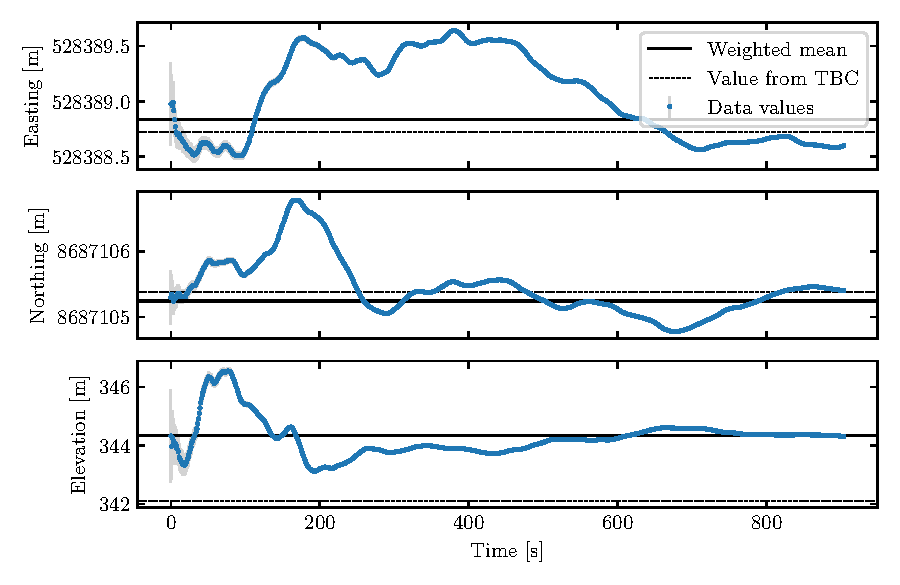
\includegraphics[width=\textwidth]{./figs/timeseries/46250723_corr-T1-ii-2017_Timeseries-east-north-elev.pdf}
    \caption{Second measurement  of two measurements of position of stake T1-2017  after the open source processing. The blue points are the open source values Northing, Easting and Elevation in m in respect to the measurement time in s. The solid black line is the weighted mean of the open source values. The dashed line is the Trimble Business Center value for the same stake. The gray shadowed range shows the uncertainty area.}
    \label{GPS:fig:T1-ii_timeseries}
\end{figure}

\subsection{Stake correction}
The post processed data with the base station data are not the final position data. 
Finally, the differences due to the measurement set up has to be considered by tge stake correction include the different aspects from our measurement setup (see sec. \ref{GPS:subsec:setup}).
The distance between the rover and the stake has to be subtracted from the northing component.
Also it was necessary to correct the position on the ice surface with the inclination of the stake. 
For this, we consider the inclination of the stake and calculate the error dependent on the height of the stake and the direction of the inclination.
The measurement data which are relevant for our stake corrections are in the appendix in table \ref{GPS:tab:fb_other_tab}.
For the better understanding all variables for the stake corrections are shown in the schematic figure \ref{GPS:fig:scheme}.

\begin{figure}[H]
	\centering
	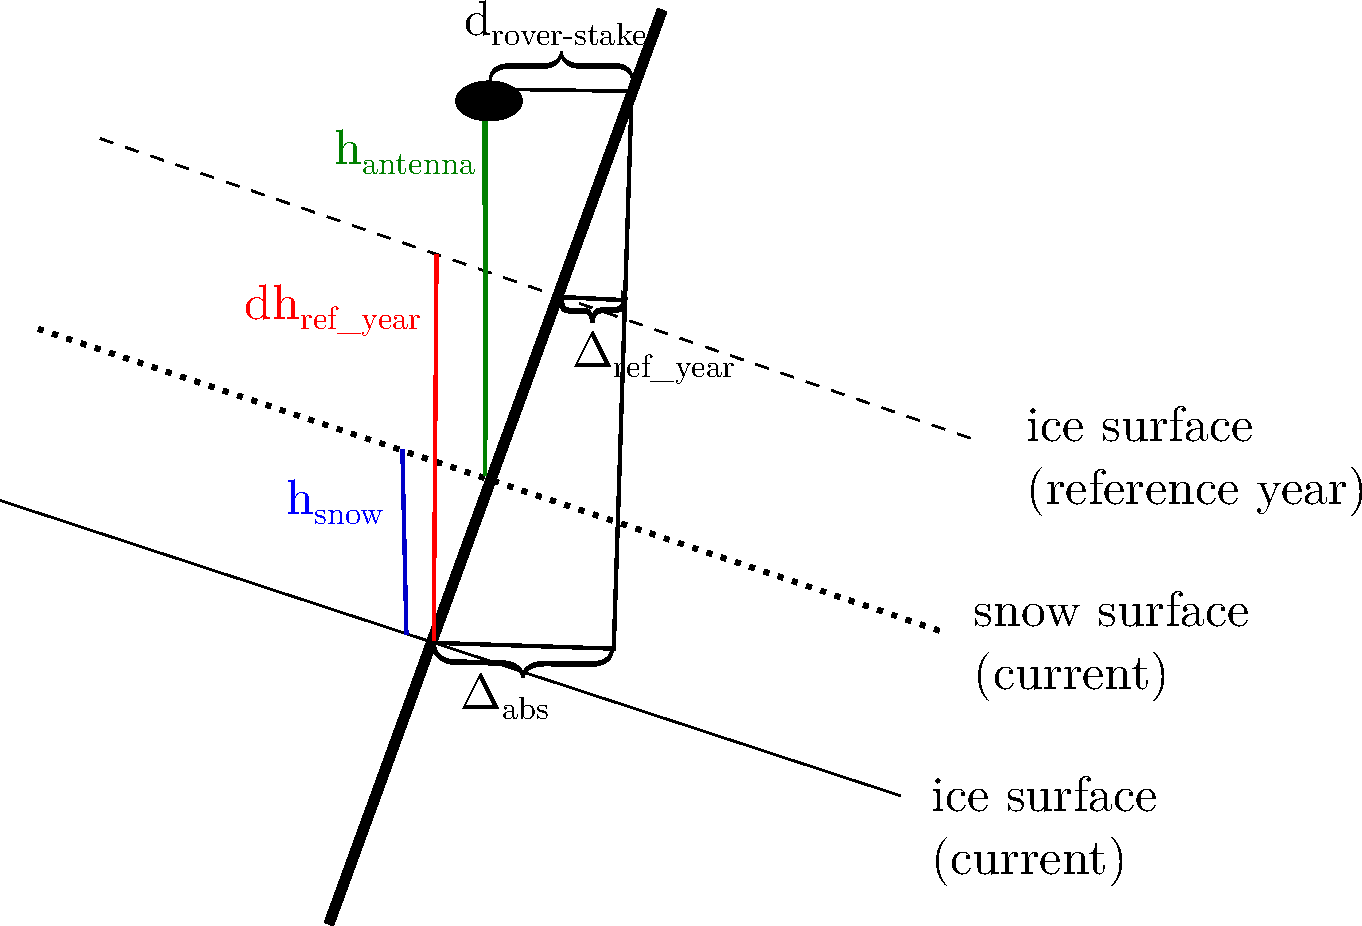
\includegraphics[width=0.9\linewidth]{./figs/pictures/schematic_setup.pdf}
	\caption{Schematic figure with the setup and the relevant parameter for the stake correction and velocity calculation. The thick tilted line is the mass balance stake and the oval object is the rover. The dashed line shows the ice surface for the referenced year. The dotted line shows the snow surface and the solid line the ice surface of this year. The colored distances are the snow height $h_{\text{snow}}$ (blue), antenna height $h_{\text{antenna}}$ (green) and the ice surface height difference to the referenced year (red). Also the distance between rover and stake $dh_{year,2018}$ and the calculated absolut horizontal difference $\Delta_{\text{abs}}$ as well as the absolute horizontal absolute differnce to the referenced year $\Delta_{year,2018}$ are displayed in the scheme.}
	\label{GPS:fig:scheme}
\end{figure}

The stake correction is derived by the geometry of our measurement setup.
First the absolut horizontal difference $\Delta_{\text{abs}}$ depending in the inclination $\alpha$ and the height composite of snow depth $h_{\text{snow}}$ and antenna height $h_{\text{antenna}}$.
\begin{equation}
	\Delta_{\text{abs}} = (h_{\text{snow}} + h_{\text{antenna}}) * sin(\alpha)
\end{equation}

Then the correction is different for the northing and easting. The norting correction is calculated with the cosinus of the direction of the inclination $\phi$. 
The angle of direction is defined in a range from 0$^{\circ}$ to 359$^{\circ}$ with 0$^{\circ}$ for North, 90$^{\circ}$ for East, 180$^{\circ}$ for South and 270$^{\circ}$ for West.
Due to geometrical reasons the sign has to be negative. 
Additionally the the distance between the rover and the stake $d_{\text{rover-stake}}$ has to be subtracted from the original northing.
\begin{equation}
	\Delta_{\text{north}} = - (\Delta_{\text{abs}} * cos(\phi)) - d_{\text{rover-stake}}
\end{equation}

The easting difference $\Delta_{\text{east}}$ is calculated with the sine of $\phi$.
\begin{equation}
	\Delta_{\text{east}} = - \Delta_{\text{abs}} * sin(\phi)
\end{equation}

The elevation correction is different between the OS and the TCS values.
For the TBC values the elevation correction $\Delta_{\text{elev,TBC}}$ only the $h_{\text{snow}}$ need to be subtracted because the $h_{\text{antenna}}$ is already caluclated out while the measurement with the Controller.
\begin{equation}
	\Delta_{\text{elev,TBC}} = - h_{\text{snow}} 
\end{equation}

The elevation correction of the OS elevation $\Delta_{\text{elev,os}}$ is done by $h_{\text{snow}}$ and $h_{\text{antenna}}$.
\begin{equation}
	\Delta_{\text{elev,os}} = - (h_{\text{snow}} + h_{\text{antenna}}) 
\end{equation}

\subsubsection*{Referenced positions}

To calculate the actual velocity it is necessary to reference the location of the stake to the ice surface elevation of the referenced year. 
This has been done for the years 2015, 2016 and 2017 on the 2018 OS values.
In gerneal, the calculation works in the similar way.
The height for stake correction relating to the inclination is different, because the relevant height difference is changed by the height difference between this year and the refrenced year $dh_{year,2018}$ . So this variable is considered for the calculation of the absolute horizontal difference $\Delta_{year,2018}$.

\begin{equation}
	\Delta_{year,2018} = (h_{\text{snow}} + h_{\text{antenna}} - dh_{year,2018}) * sin(\alpha)
\end{equation}

\subsection{Evaluation}
For the comparison the TBC post processed coordinates are in the appendix in table \ref{GPS:tab:tbc_tab}.
For the difference between the two different methods is no bias which is proved by a small median (see table \ref{GPS:tab:diff}).
The direction of the differnce is randomly for between the stakes for all three parts of the positioning.
The differnces are mainly caused by a few unclear values after the post processing (compare table \ref{GPS:tab:diff_tab}).
Due to this the mean value for the differences is higher than the median (see table \ref{GPS:tab:diff}) 
In order that, the OS processed values are a reasonable replacement for the TBC values and are uses in the following calculatio.
This means also that the uncertainty propagation is done for the OS values so we can finaly determine the uncertainty of the velocity values.

\begin{table}[H]
	\caption{Mean and median for the difference of northing, easting and elevation between the open source and Trimble Business Center values.}
	\centering
	\begin{tabular}{lccc}
	\toprule         
      &  Northing [m] & Easting [m] & Elevation [m] \\
	\midrule
    mean difference &  0.09 & 0.05 & 0.24 \\
    median of difference & 0.01 & 0.01 & 0.09 \\
    \bottomrule
	\end{tabular}
	\label{GPS:tab:diff}
\end{table}

\subsection{Propagation of uncertainty}

The calculations for the propagation of uncertainties are done by the common rule.
The accurancy of the post processed postions with the base station data is decreasing with a increasing distance to the base station. 
But this uncertainty is at least one order of magnitude smaller than the other uncertainties and can be neglected. 
The other uncertaintied are determined by the quality of our measurements and first part of the processing (see table \ref{GPS:tab:errors}).

\begin{table}[H]
	\caption{Used uncertainty values for the propagation of uncertainty.}
	\centering
	\begin{tabular}{lc}
	\toprule
        uncertainty &  value \\
	\midrule
    $ \delta_{\alpha} $ &  3$^{\circ}$ \\
    $ \delta_{\phi} $ &  22.5$^{\circ}$ \\
    $ \delta_{h_{snow}}$ &  0.02 m \\
    $ \delta_{h_{antenna}} $ &  0.05 m \\
    $ \delta_{dh_{year,2018}} $ &  0.10 m \\
    $ \delta_{d_{rover-stake}} $ &  0.02 m \\
    $ \overline{\delta_{\text{N}}} $ & 0.40 m \\
    $ \overline{\delta_{\text{E}}} $ & 0.19 m \\
    $ \overline{\delta_{\text{H}}} $ & 0.89 m \\
    \bottomrule
	\end{tabular}
	\label{GPS:tab:errors}
\end{table} 

The uncertainty of the absolut horizontal difference $\delta_{\Delta_{\text{abs}}}$ is dependent on the uncertainties of the parameter and the parameter itself.
\begin{equation}
	\delta_{\Delta_{\text{abs}}} = \sqrt{(h_{\text{snow}} + h_{\text{antenna}})^2 * \delta_{\alpha}^2 * cos^2(\alpha) + (\delta_{h_{\text{snow}}}^2 + \delta_{h_{\text{antenna}}}^2) * \sin^2(\alpha)}
\end{equation}

The uncertainty of the northing correction $\delta_{\Delta_{\text{north}}}$ is
\begin{equation}
	\delta_{\Delta_{\text{north}}} = \sqrt{\delta_{\Delta_{\text{abs}}}^2 * cos^2(\phi) + \Delta_{\text{abs}}^2 * \delta_{\phi}^2 * sin^2(\phi) + \delta_{d_{\text{rover-stake}}}^2}
\end{equation}

The uncertainty of the easting correction $\delta_{\Delta_{\text{east}}}$ is
\begin{equation}
	\delta_{\Delta_{\text{east}}} = \sqrt{\delta_{\Delta_{\text{abs}}}^2 * sin^2(\phi) + \Delta_{\text{abs}}^2 * \delta_{\phi}^2 * cos^2(\phi)}
\end{equation}

The uncertainty of the elevation correction $\delta_{\Delta_{\text{elev}}}$ is
\begin{equation}
\delta_{\Delta_{\text{elev}}} = \sqrt{\delta_{h_{\text{snow}}}^2 + \delta_{h_{\text{antenna}}}^2}
\end{equation}
	
Based on this uncertainties the total uncertainty for norting $\delta_{\Delta_{\text{total,north}}}$, easting $\delta_{\Delta_{\text{total,east}}}$ and eleavtion $\delta_{\Delta_{\text{total,elev}}}$ can calculated with the uncertainty of the time series of our OS post processed GPS time series $\delta_{\Delta_{\text{ts,north}}}$ for northing, $\delta_{\Delta_{\text{ts,east}}}$ for easting and $\delta_{\Delta_{\text{ts,elev}}}$ for the elevation.
\begin{equation}
	\delta_{\Delta_{\text{total,north}}} = \sqrt{\delta_{\Delta_{\text{ts,north}}}^2 + \delta_{\Delta_{\text{north}}}^2}
	\label{GPS:eq:errnorth}
\end{equation}

\begin{equation}
	\delta_{\Delta_{\text{total,east}}} = \sqrt{\delta_{\Delta_{\text{ts,east}}}^2 + \delta_{\Delta_{\text{east}}}^2}
	\label{GPS:eq:erreast}
\end{equation}

\begin{equation}
	\delta_{\Delta_{\text{total,elev}}} = \sqrt{\delta_{\Delta_{\text{ts,elev}}}^2 +\delta_{\Delta_{\text{elev}}}^2}
	\label{GPS:eq:errnelev}
\end{equation}

\subsubsection*{Referenced positions}

For the refenced positions only two euations differ to the previous uncertainty propagation. 
The uncertainty of the absolute difference $\Delta_{year,2018}$ is
\begin{equation}
\begin{split}
\delta_{\Delta_{year,2018}} = & 
\ ((h_{\text{snow}} + h_{\text{antenna}} - dh_{year,2018})^2 * \delta_{\alpha}^2 * cos^2(\alpha)\\
&+ (\delta_{h_{\text{snow}}}^2 + \delta_{h_{\text{antenna}}}^2 + \delta_{dh_{year,2018}}^2) * \sin^2(\alpha))^{1/2}
\end{split}
\end{equation}

The uncertainty for the elevation correction $\delta_{\Delta_{year, \text{elev}}}$ is also different by the uncertainty of the height difference of the ice surface $\delta_{dh_{\text{year, 2018}}}$.
\begin{equation}
	\delta_{\Delta_{year, \text{elev}}} = \sqrt{\delta_{h_{\text{snow}}}^2 + \delta_{h_{\text{antenna}}}^2 + \delta_{dh_{\text{year, 2018}}}^2}
\end{equation}

\subsection{Final positions}

The final positions are based on the open source post processing and stake correction.
This position values decribe the position on the elevation of the ice surface. 
The corresponding uncertainties for each value are determined by the calculation of uncertainties (eq. \ref{GPS:eq:errnorth} - \ref{GPS:eq:errnelev}). 
This values and uncertainties in table \ref{GPS:tab:os_tab} are used in the next section to determine the velocities at the different stake locations. 

\begin{table}[H]
	\caption{Final positions with Northing, Easting and Elevation for every stake after the open source post processing and stake correction with the corresponding error.}
	\centering
	\begin{tabular}{lrrrrrr}
\toprule
        Name &  Northing [m] &  Error Northing [m] &  Easting [m] &  Error Easting [m] &  Elevation [m] &  Error Elevation [m] \\
\midrule
    BL2-2016 &    8686150.74 &                0.16 &    523049.41 &               0.11 &         436.89 &                 0.48 \\
    BL2-2018 &    8686149.82 &                0.01 &    523051.47 &               0.03 &         437.74 &                 0.06 \\
    BL3-2016 &    8686091.51 &                0.27 &    523544.75 &               0.13 &         490.82 &                 0.25 \\
    BL3-2018 &    8686091.17 &                0.42 &    523545.34 &               0.10 &         491.39 &                 1.03 \\
    BL4-2018 &    8686098.58 &                0.17 &    524179.27 &               0.15 &         573.74 &                 0.20 \\
  BL4-i-2016 &    8686098.47 &                0.26 &    524179.80 &               0.19 &         571.65 &                 0.20 \\
 BL4-ii-2016 &    8686098.39 &                1.30 &    524179.92 &               0.31 &         571.36 &                 4.82 \\
  BL5-i-2017 &    8686130.74 &                0.09 &    524644.27 &               0.01 &         628.63 &                 0.09 \\
 BL5-ii-2017 &    8686130.74 &                0.28 &    524644.28 &               0.15 &         628.56 &                 0.75 \\
     T1-2018 &    8687106.55 &                0.32 &    528388.42 &               0.07 &         341.59 &                 0.24 \\
   T1-i-2017 &    8687105.69 &                0.13 &    528388.68 &               0.18 &         341.26 &                 0.12 \\
  T1-ii-2017 &    8687105.58 &                0.45 &    528388.84 &               0.44 &         341.38 &                 0.65 \\
     T2-2016 &    8687321.31 &                0.42 &    527951.88 &               0.14 &         394.88 &                 2.34 \\
     T2-2018 &    8687319.62 &                0.28 &    527951.35 &               0.27 &         395.86 &                 1.61 \\
   T2-i-2017 &    8687321.37 &                0.30 &    527950.58 &               0.25 &         395.22 &                 0.34 \\
  T2-ii-2017 &    8687320.98 &                1.31 &    527951.01 &               0.26 &         394.74 &                 1.26 \\
     T3-2017 &    8687273.11 &                0.11 &    527598.29 &               0.01 &         422.59 &                 0.07 \\
     T4-2016 &    8687138.56 &                0.47 &    527123.97 &               0.34 &         486.80 &                 1.07 \\
     T4-2018 &    8687137.72 &                1.05 &    527124.90 &               0.37 &         487.94 &                 2.33 \\
     T5-2016 &    8686938.28 &                0.57 &    526692.25 &               0.25 &         534.57 &                 0.72 \\
     T5-2018 &    8686937.68 &                0.21 &    526690.76 &               0.21 &         535.09 &                 0.45 \\
     T6-2016 &    8686675.01 &                0.51 &    526250.17 &               0.22 &         561.87 &                 0.89 \\
     T6-2018 &    8686674.78 &                0.48 &    526246.88 &               0.39 &         560.47 &                 0.79 \\
     T7-2015 &    8686578.89 &                0.24 &    525858.01 &               0.17 &         615.10 &                 0.71 \\
     T7-2017 &    8686579.37 &                0.19 &    525858.38 &               0.04 &         615.95 &                 0.71 \\
     T8-2017 &    8686471.52 &                0.48 &    525523.82 &               0.13 &         649.73 &                 1.02 \\
\bottomrule
\end{tabular}

	\label{GPS:tab:os_tab}
\end{table}
